\section{The nonlinear vacuum carrier and the rank-3 Wilczek--Zee bundle}
\label{sec:carrier}

The central result is that the fluctuation operator about a finite-amplitude periodic
background carries an isolated rank-3 complex eigenbundle whose Wilczek--Zee curvature
generates the full algebra $\su{3}$.

\subsection{The carrier and the criterion}

Following the chain of Section~\ref{sec:substrate}, a stationary periodic background $\bar R$
gives stiffness tensors $C_{n\mu}[\bar R]$ and a Bloch operator $D_{\bar R}(\veck)$. The
color sector requires an \emph{isolated rank-3} spectral subspace $P_3(\veck)$---a
near-degenerate triplet $\lambda_1\approx\lambda_2\approx\lambda_3$ with a large outside gap
$\varepsilon\ll\Delta$ (a composite subspace, not exact degeneracy)---transported nontrivially
over the base. On $P_3$ the non-abelian Wilczek--Zee connection and its gauge-invariant
curvature are
\begin{equation}
  [\Ac_\mu]_{ab}=\ii\langle\varepsilon_a|\partial_{k_\mu}\varepsilon_b\rangle,\qquad
  \Fc_{\mu\nu}=\ii P_3[\partial_{k_\mu}P_3,\partial_{k_\nu}P_3]P_3,
  \label{eq:wz}
\end{equation}
with the algebraic split $\Ac_\mu=a_\mu I_3+B_\mu$, $\Tr B_\mu=0$, so
$\Fc_{\mu\nu}=f_{\mu\nu}I_3+\Gc_{\mu\nu}$ ($\uu{3}\simeq\uu{1}\oplus\su{3}$). The connection
is $\uu{3}$-valued because the transported carrier is rank $3$ over a 4D base: four-dimensional
$\mu,\nu$ indices do not enlarge the internal group. The natural rank-3 carrier is the
complexified transverse-fluctuation bundle: at each link the direction $\Qhat\in\R^4$ leaves a
three-dimensional orthogonal complement, which Bloch-complexifies to $\C^3$; this moving
triplet, not the fixed spatial axes, is the color-carrier candidate. The sharp test is
\begin{equation}
  \Lie\bigl\langle \Gc_{\mu\nu},\ [\Gc_{\mu\nu},\Gc_{\rho\sigma}],\ \dots\bigr\rangle
  \;\stackrel{?}{=}\;\su{3}\quad(\text{real dimension }8),
  \label{eq:criterion}
\end{equation}
distinguishing genuine $\su{3}$ (rank $8$) from the real-frame $\mathfrak{so}(3)$ (rank $3$)
or a pure-gauge $\uu{3}$ artifact (rank $0$). Gauge invariance is essential and is enforced by
computing $\Fc_{\mu\nu}$ with the Wilson-loop (Fukui--Hatsugai) construction
\citep{FukuiHatsugai2005}, which is manifestly invariant under $k$-local $U(3)$ basis changes.

\subsection{An exact stationary carrier}
\label{subsec:carrier-construct}

We use a closed-form circularly-polarized helix,
\begin{equation}
  \bar R_n=a\,n+A\bigl[\cos(K\!\cdot\!n)\,p+\sin(K\!\cdot\!n)\,q\bigr],\qquad
  K=(K_1,0,0,K_4),\ p=\hat e_2,\ q=\hat e_3,
  \label{eq:helix}
\end{equation}
with propagation in the $(1,4)$ plane and polarization in the $(2,3)$ plane. Because
$\operatorname{span}(p,q)\perp\hat e_1,\hat e_4$ and $K$ has no component along $2,3$, every
link length is independent of $n$ (transverse increments are chords of a fixed angle), while
the link directions $\Qhat_{n1},\Qhat_{n4}$ twist with $n$. All link tensions are then
constant, and the nodal force reduces to a single transverse condition; the spatial
($\rho_1<0$) and temporal ($\rho_4>0$) contributions have opposite sign precisely because of
the Lorentzian pattern~\eqref{eq:eta}, so a positive $\gamma_t$ solves the balance. The result
is an \emph{exact} critical point: the numerical residual is $\|\nabla S\|\approx 2\times10^{-16}$
\citep{repo}. This is a genuine finite-amplitude nonlinear periodic state of the lattice, in
compliance with periodic boundary conditions.

\subsection{Result: full $\su{3}$}
\label{subsec:su3}

\begin{figure}[t]
  \centering
  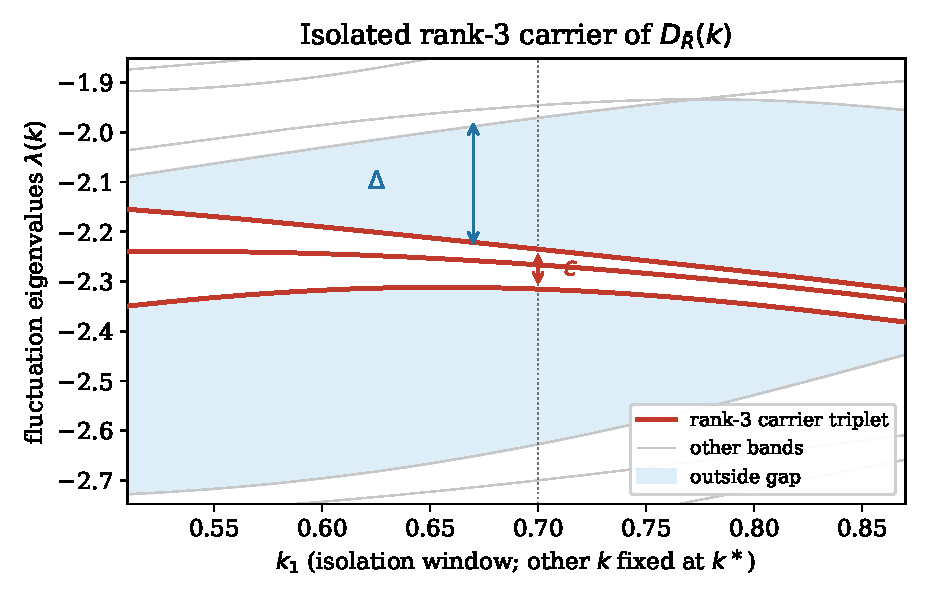
\includegraphics[width=0.72\textwidth]{figures/fig_bands}
  \caption{Fluctuation spectrum of the Bloch operator $D_{\bar R}(k)$ along a
  $k_1$-cut through the reference point $k^\ast$ (dotted line; other components fixed at
  $k^\ast$), over the window where the carrier stays isolated. The rank-3 carrier triplet
  (bold red) is a near-degenerate composite---small internal spread $\varepsilon$ (red
  arrow) with a large outside gap $\Delta$ (blue arrow) to the remaining bands
  (gap/spread $\approx 3.3$)---so the projector $P_3(k)$ is well defined. Isolation is
  local (a near-degenerate composite; see Section~\ref{subsec:generic}), as
  reflected by the finite window.}
  \label{fig:bands}
\end{figure}

Running the chain on the carrier~\eqref{eq:helix} at, e.g., $(\alpha_s,\alpha_t,A)=(0.6,0.9,0.3a)$,
$N_1=N_4=3$ (which fixes $\gamma_t\approx 2.32$), an isolated rank-3 cluster is found with
gap/spread $\approx 3.3$ (Figure~\ref{fig:bands}). The gauge-invariant curvature yields
\begin{equation}
  \text{so(3) span}=3/3,\quad \text{sym.+Cartan span}=5/5,\quad
  \text{raw span}=8/8,\quad \boxed{\text{Lie-closure rank}=8}\ \ (\su{3}),
\end{equation}
while the trace curvature is numerically zero ($|\Tr\Fc|\sim 10^{-11}$): this symmetric carrier
gives \emph{pure color}, with the traceless part unambiguously $\su{3}$-valued
\citep{repo}. The eight generators are populated \emph{before} any commutator is taken (raw
span already $8$).

\paragraph{Mechanism ($\mathfrak{so}(3)\to\su{3}$).} A control isolates the mechanism
(Figure~\ref{fig:su3}b). A real transverse frame (a single-site real-symmetric operator) gives
raw span $3$, Lie rank $3$: only $\mathfrak{so}(3)$. Removing all $k$-transport gives rank $0$
(trivial bundle); restoring the complex Bloch phases gives rank $8$: the three antisymmetric
$\mathfrak{so}(3)$ generators come from orientation transport of the real frame, and the five
symmetric-traceless $+$ Cartan generators that complete $\su{3}$ come from the \emph{complex
Bloch phases} acting on the noncommuting real stiffness frames \citep{repo}. This resolves the
long-standing $\mathfrak{so}(3)$-vs-$\su{3}$ question: complex phases on a genuine (multi-site)
supercell background are the necessary ingredient. Because the base and substrate remain 4D while only the transported carrier is
rank $3$, the group is $U(3)$, never $SU(4)$ (Section~\ref{sec:split}).

\subsection{Genericity, scaling, and consistency}
\label{subsec:generic}

\begin{figure}[t]
  \centering
  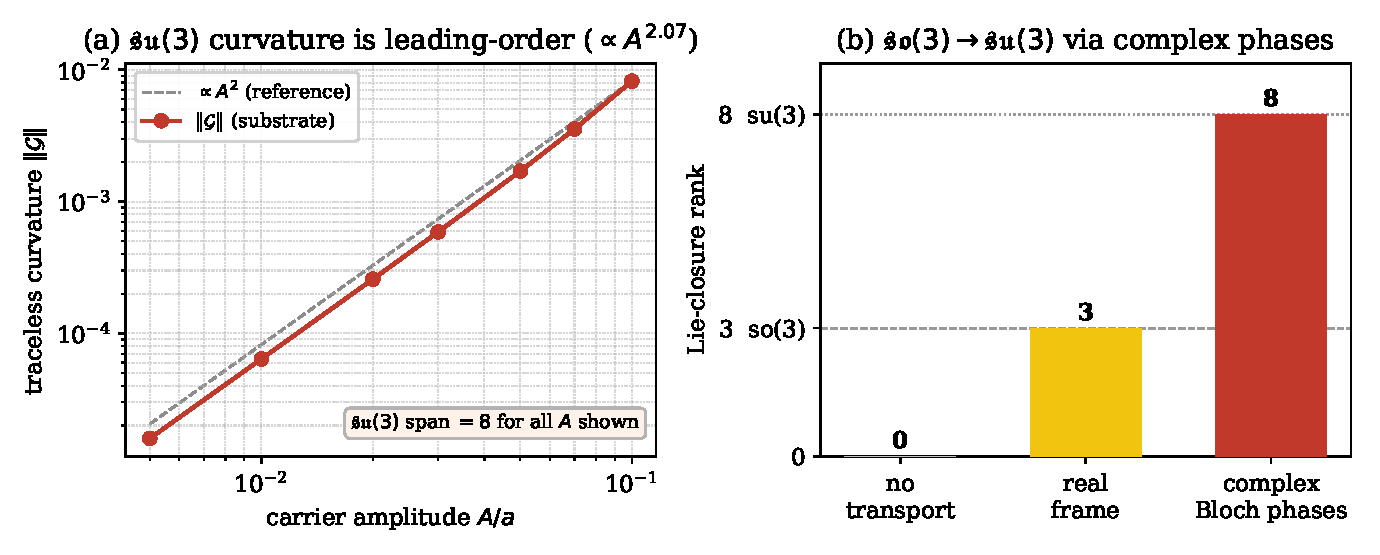
\includegraphics[width=0.98\textwidth]{figures/fig_su3}
  \caption{(a)~Small-amplitude scaling: the traceless curvature magnitude
  $\|\Gc_{\mu\nu}\|$ (fixed band and $k^\ast$) follows the reference $\propto A^2$ line over more
  than a decade in carrier amplitude, and the $\su{3}$ span stays $8$ down to $A=0.005$---so the
  $\su{3}$ is a leading-order effect that vanishes continuously in the flat-vacuum limit, not a
  large-amplitude artifact. (b)~The $\mathfrak{so}(3)\to\su{3}$ mechanism: with no $k$-transport
  the bundle is trivial (rank $0$); a real moving frame gives only $\mathfrak{so}(3)$ (rank $3$);
  the complex Bloch phases of a genuine supercell background complete the algebra to $\su{3}$
  (rank $8$).}
  \label{fig:su3}
\end{figure}

Three checks upgrade the single witness to a robust, generic result \citep{repo}:
\begin{itemize}
  \item \textbf{Genericity.} Over $24$ distinct exact-stationary helices (varying propagation
  axis, supercell size, winding, $\alpha_s,\alpha_t$, amplitude; all $\|\nabla S\|\lesssim10^{-15}$),
  the robust Lie rank is $8$ in $23/24$ cases; the lone exception is a
  measure-zero, $k^\ast$-specific accident, exactly as a genericity argument predicts (a set of traceless
  Hermitian matrices fails to generate $\su{3}$ only if it lies in a proper subalgebra, a
  positive-codimension condition). The result is also stable across supercell size and
  plaquette step.
  \item \textbf{Leading-order scaling} (Figure~\ref{fig:su3}a). The $\su{3}$ span persists down to
  carrier amplitude $A=0.005$; tracking a fixed band/plaquette gives $\|\Gc\|\sim A^{2.07}$ (leading order $A^2$),
  while the mechanical seed---stiffness-matrix noncommutativity---scales as
  $\|[C,C]\|\sim A^{0.90}$ (order $A$). This matches $\partial_k P_3\sim O(A)\Rightarrow
  \Fc\sim(\partial P)^2\sim O(A^2)$, with the complex phases (order $1$) supplying all eight
  directions already at that order. The $\su{3}$ is thus a leading-order effect, not a
  large-amplitude artifact, and vanishes continuously as $A\to 0$.
  \item \textbf{Bianchi.} In a parallel-transport gauge the relative residual
  $\|D_{[\mu}\Gc_{\nu\rho]}\|/\|\Gc\|$ falls as $O(h^2)$ (from $1.1\times10^{-4}$ to
  $6.8\times10^{-6}$): the non-abelian Bianchi identity holds, confirming $\Gc$ is a consistent
  curvature.
\end{itemize}
Together these establish that the substrate's own curvature generates the full $\su{3}$ as a
generic, discretization-robust, leading-order, identity-satisfying property---not a tuned or
numerical artifact.
